Lo sviluppo tecnologico nel campo dell'intelligenza artificiale ha permesso una grande evoluzione nel campo della guida autonoma. L'interesse per questo 
settore è guidato dai seguenti vantaggi che questi veicoli possono potenzialmente portare\cite{advantages}:
\begin{itemize}
    \item \textbf{Riduzione degli incidenti} Una grossa parte degli incidenti stradali(fino al $90\%$ )sono dovuti a errori umani. Eliminarli
    significherebbe ridurre notevolmente il numero di infortuni e salvare delle vite.
    \item \textbf{Riduzione del traffico} Grazie al controllo automatico si possono evitare le situazioni di congestione che avvengono naturalmente sulle strade.
    Oltre a migliorare il deflusso veicolare, questo porterebbe anche  una riduzione delle emissioni di CO2 e del consumo di benzina, causate dalle macchine ferme nel traffico.
    \item \textbf{Migliore capacità stradale} L'ottimizzazione del trafico potrebbe portare un notevole incremento nella capacità autostradale. La capacità
    di monitorare in modo costante l'ambiente circostante e reagire istantaneamente renderebbe più sicuro viaggiare a velocità maggiori e con meno spazio tra ciascun veicolo.
    \item \textbf{Accessibilità} Attualmente  molte persone anziane  e/o con disabilità sono escluse dal viaggio in automobile in solitaria. Le self-driving car rappresentano un'opportunità
    di indipendenza per queste categorie, che potrebbero così muoversi senza dover ricorrere a soluzioni esterne.
\end{itemize}
Attualmente però non si puo parlare ancora di guida completamente autonoma, ma di sistemi di guida assistita. Restano ancora molte problematiche aperte, soprattutto 
da un punto di vista legale\cite{legal} etico\cite{Lin2015}. Per questo, e per i problemi di \emph{safety} e \emph{dependability} che verrano illustrati nei prossimi paragrafi, lo sviluppo
di veicoli autonomi è in molti casi ancora in fase prototipale. La ricerca è quindi fondamentale per portare a miglioramenti significativi.
\section{Livelli di automazione}
Nel 2014 la \textbf{SAE international} ha pubblicato lo standard J3016, col quale vengono definiti sei liveli di autonomia, in base a quanto un guidatore deve intervenire.
\begin{figure}
    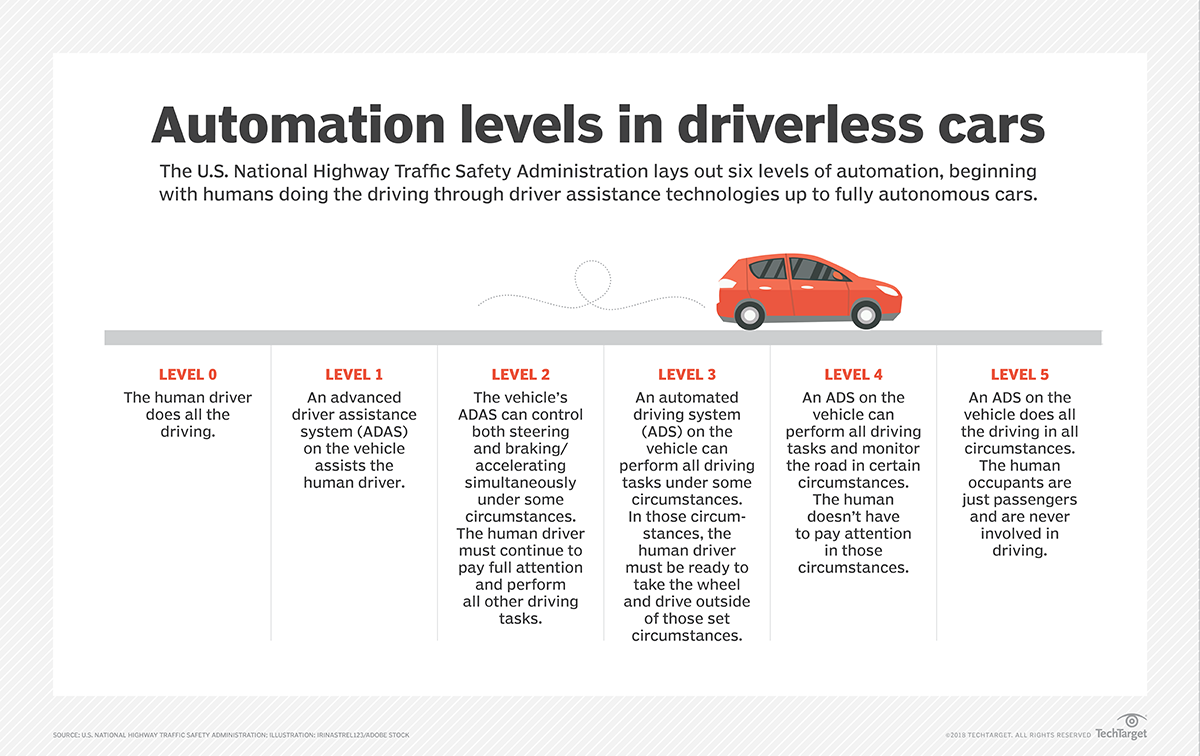
\includegraphics[width=\linewidth]{car_automation_levels.png}
    \caption{livelli di automazione\cite{car}}
    \label{fig:adaslevel}
\end{figure}
\subsubsection{Livello 0}
Nessun tipo di automazione. Il controllo è completamente affidato al conducente.
\subsubsection{Livello 1: Assistenza alla guida}
Il conducente si occupa di tutti gli aspetti della guida. Viene supportato da sistemi elettronici che possono  segnalare la presenza di pericoli attraverso segnali visivi e acustici.
Vengono classificati di livello 1 anche i veicoli con una singola funzione di assistenza automatizzata(ad esempio il controllo automatico della velocità).
\subsubsection{Livello 2: Automazione Parziale}
Il conducente deve mantenere il controllo del veicolo in ogni istante ma le le varie funzioni vengono automatizzate da 
due o più sistemi avanzati di assistenza alla guida(\textbf{sistemi ADAS}). Questi sistemi includono:
\begin{itemize}
    \item Adaptive Cruise Control- controllo automatico della velocità
    \item Lane-Keeping Assist - controllo dello sterzo per impedire l'uscita dalla corsia
    \item Automatic Emergency Braking -  controllo del freno per le situazioni di emergenza
\end{itemize}
\subsubsection{Livello 3: Automazione condizionale}
La guida è completamente automatizzata ma non in tutti i momenti del viaggio. IL conducente viene avvisato quando deve riprendere il controllo ed è tenuto a rispondere
in modo appropriato. Se questo non avviene, il sistema arresta il veicolo nel modo più sicuro possibile
\subsubsection{Livello 4: Alta Automazione}
Il viaggio è completamente gestito dal sistema. Il conducente non è tenuto a intervenire in nessun momento. La completa autonomia è garantita però a patto che non esistano limitazioni come ad esempio condizioni
metereologiche fortemente avverse.
\subsubsection{Livello 5: Automazione totale}
Sistema completamente autonomo. Non vi è alcuna limitazione ed è tutto gestito dal sistema interno in qualunque momento. Attualmente sono in commercio solamente veicoli appartenenti ai livello 0-2 mentre esistono solamente prototipi di livello 3 e 4. Il livello 5 è ancora molto lontano, forse irragiungibile, tant'è che
molti esperti credono che sia molto più importanti concentrarsi sullo sviluppo di livello 4.
